\subsection{Topology Discovery Protocol}
\label{proto_topo}

The \dcamp distributed topology is dynamically established as the Root node sends out its discovery message and receives
join messages from Base nodes. Once a Base node responds to the Root, the Base node is given its assignment.

\begin{figure}[ht]
    \centering
    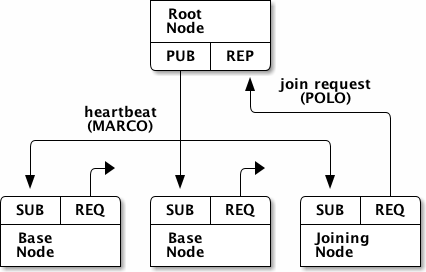
\includegraphics[scale=0.66]{topo.png}
    \label{fig:proto_topo_image}
    \caption{Topology Discovery Protocol Diagram}
\end{figure}

\begin{figure}[ht]
\vspace{+10pt}
\begin{verbatim}
topo-discovery = *discover join
discover       = R-MARCO
join           = B-POLO ( R-ASSIGN / R-WTF )
\end{verbatim}
\vspace{-5pt}
\caption[Topology Discovery Protocol]
        {Topology Discovery Protocol: \texttt{R-} represents the Root node sending a message and \texttt{B-}
         represents a Base node sending a message.}
\label{fig:proto_topo_spec}
\end{figure}

\subsubsection{Message Definitions}

\textbf{MARCO} \\
discovery message, two frames

\begin{verbatim}
Frame 0: root endpoint identity, as 0MQ string
Frame 1: root endpoint UUID, 16 bytes in network order
\end{verbatim}

\textbf{POLO} \\
join message, two frames

\begin{verbatim}
Frame 0: base endpoint identity, as 0MQ string
Frame 1: base endpoint UUID, 16 bytes in network order
\end{verbatim}

\textbf{CONTROL} \\
control message, two frames; frame 1 contains the specific topology instructions (level-one collector, leaf node, etc.)

\begin{verbatim}
Frame 0: command, as 0MQ string
Frame 1: properties, JSON-encoded, as 0MQ string
command     = "assignment" / "stop"
properties  = *( parent / level / group / config-file )
parent      = "parent=" <node-endpoint-identity>
level       = "level=" ( "root" / "branch" / "leaf" )
group       = "group=" <group-identity> / NULL
config-file = "config-file=" <file-path>
\end{verbatim}

\textbf{WTF} \\
error message, three frames (the error string may be empty)

\begin{verbatim}
Frame 0: "WTF"
Frame 1: error code, 4 bytes in network order
Frame 2: error message, as 0MQ string
\end{verbatim}
